\documentclass{article}
\usepackage[utf8]{inputenc}
\usepackage{hyperref}
\usepackage{amsmath}
\usepackage{amsfonts}
\usepackage{graphicx}
\usepackage{enumitem}
\usepackage{wrapfig}
\graphicspath{ {./images} }


\title{Introduction to Forces}
\author{
    Tan Chien Hao\\
    \texttt{www.tchlabs.net}\\
    \texttt{Telegram @tch1001}
    % new collaborators add your name and contact here!
}

\date{\today}
\begin{document}
\newif\ifpaper

% TOGGLE ANSWER HERE
\paperfalse 

\maketitle
\section{Forces}
What is a force?
\begin{itemize}
    \item A force causes acceleration
    \item Forces are vectors, meaning they have both magnitude and direction
    \item Units of force is \textbf{Newton} (N). 1 N = 1 kg $\times$ $1\mathrm{~m} / \mathrm{s}^2$
    \item Contact vs Non-contact
    \item Attractive vs Repulsive
    \item *Conservative vs Non-conservative
    \item *Real vs Fictitious
\end{itemize}
* means more advanced concept\\[10pt]
\noindent Examples of Forces
\begin{itemize}
    \item Normal contact force
    \item Gravitational Force
    \item Tension
    \item Magnetic Force
    \item Electrostatic Force
    \item Centrifugal Force
    \item Drag 
    \item Friction
    \item Strong Nuclear Force
    \item Spring Force
\end{itemize}

\section{Newton's Laws of Motion}
Newton postulated the following laws according to experimental observation.

\subsection{Newton's 1st Law}
In an \textbf{inertial} reference frame, if a body is at rest or moving at a constant speed in a straight line, it will remain at rest or keep moving in a straight line at constant speed unless it is acted upon by a force. \\[10pt]
\noindent In other words, $F = 0$ implies $a = 0$. 

\subsection{Newton's 2nd Law}
The acceleration $a$ of an object is equals to the net force acting on it, divided by it's mass.
\begin{align}
    a = \frac{F_\text{net}}{m}
\end{align}

\noindent Important: cause and effect. The force \textbf{causes} acceleration. 

\subsection{Newton's 3rd Law}
Every force has an equal and opposite reaction
\begin{align}
    F_{\text{A on B}} = -F_{\text{B on A}}
\end{align}

\noindent The fact that their absolute value is the same reflects the fact that both forces have \textbf{equal magnitude}. The minus sign reflects \textbf{opposite direction}. \\[10pt]
\noindent Examples: 
\begin{itemize}
    \item Gravitational force between you and the earth
    \item Firing a bullet
    \item Normal contact force between book and table
    \item *Tension in rope segments
\end{itemize}

\noindent Extra: Note this doesn't hold true for Lorentz force in electromagnetism. But we don't need to worry about this for now.

\section{Gravitational Force}
\textbf{Gravitational field}: A region of space where a mass experiences a force due to the gravitational attraction of another mass. For example, Earth's gravitational field causes objects (like the Moon) to be attracted to earth. \\[10pt]
On the surface of Earth, the \textbf{gravitational force} is always downwards with magnitude of 
\begin{align}
    W = F_{\text{grav}} = -mg
\end{align}
(assuming we take upwards as positive). Earth's \textbf{gravitational field strength} is $g=9.81 \mathrm{~m} / \mathrm{s}^2 = 9.81 \mathrm{~N} / \mathrm{kg}$. \\[10pt]
\noindent On a different planet, $g=9.81 \mathrm{~m} / \mathrm{s}^2$ would be replaced with another value $g_{\text{planet}}$. For example, on earth's moon, $g_{\text{moon}} = 1.62 \mathrm{~m} / \mathrm{s}^2$. \\[10pt]
\noindent This means that although \textbf{mass is same} on different planets, \textbf{weight is different}.
\begin{figure}[h]
    \centering
    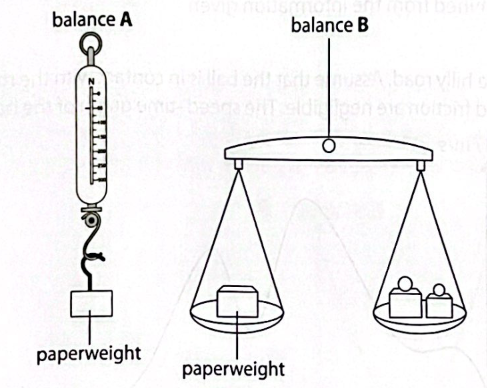
\includegraphics[width=\linewidth]{images/springbalance.png}
    \caption{Spring Balance and Scale balance}
    \label{fig:enter-label}
\end{figure}

\noindent A spring balance \textbf{measures} the weight of an object, in units of N (Newtons).\\[5pt]
A scale balance \textbf{compares} the weight of 2 objects. It tips towards the heavier one.

\subsection{Free Fall due to Gravity}
In the absence of other forces besides gravitational force, acceleration $a$ will downwards, with magnitude being the gravitational field strength $g$. Taking upwards as positive,
\begin{align}
    F_\text{net} &= F_\text{grav} = -mg \\
    \text{Using } F_\text{net} &= ma \\
    \Rightarrow ma &= -mg \\
    a &= -g
\end{align}
Neil Armstrong Video \href{https://youtu.be/Oo8TaPVsn9Y}{https://youtu.be/Oo8TaPVsn9Y}

\section{Pressure}
Pressure is the force applied \textbf{perpendicular} to the surface of an object \textbf{per unit area} over which that force is distributed.
\begin{align}
    P = \frac{F}{A}
\end{align}
Examples:
\begin{itemize}
    \item Box on a table
    \item Gas in a container
    \item Steve Splanger Video \href{https://youtu.be/zlDaIsKm6so}{https://youtu.be/zlDaIsKm6so}
    \item *Light shining on solar sail
\end{itemize}

\subsection{Hydraulics}
The hydraulic fluid in a hydraulic cylinder has approximately (up to minor height differences) constant pressure everywhere. Hydraulics work by having different areas for the pistons. 
\begin{align}
    \frac{F_1}{A_1} =\ & P = \frac{F_2}{A_2} \\
    \Rightarrow \quad \frac{F_1}{F_2} &= \frac{A_1}{A_2} 
\end{align}

\subsection{Atmospheric Pressure}
Atmospheric pressure is the pressure the atmosphere of Earth (air) exerts on objects. Over long distance scales, atmospheric pressure decreases the higher we go. The reason behind this is that air has mass. \\[10pt]
Intuition: Ball Pit analogy \\[10pt]
We will go through the math derivation in future after we learn calculus.

\end{document}